% DO NOT COMPILE THIS FILE DIRECTLY!
% This is included by the other .tex files.

\begin{frame}[t,plain]
\titlepage
\end{frame}

\begin{frame}{The bright side of information sharing}
\begin{itemize}
        \item We build various information sharing communities (one is more than 1500 organisations with more than 4000 users). {\bf sharing and updating daily cybersecurity indicators, financial indicators or threats in both ways}
        \item To achieve this we actively develop, maintain and support MISP (an open source threat sharing\footnote{also called TIP, CTI platform. \url{http://www.misp-project.org}} platform)
        \item Beside the tools, {\bf practices, standard formats and classifications} play an important role
        \item These practices need to be shared among the communities to support efficient collaboration
\end{itemize}
\end{frame}

\begin{frame}
\frametitle{How to be successful in building an information sharing community?}
        {\center \it \Huge There was never a plan. There was just a series of mistakes.\\}
        \begin{flushright}
        Robert Caro, journalist.
        \end{flushright}
\end{frame}


\begin{frame}
 \frametitle{MISP and starting from a practical use-case}
 \begin{itemize}
         \item During a malware analysis workgroup in 2012, we discovered that we worked on the analysis of the same threat actor
         \item We wanted to share information in an easy and automated way {\bf to avoid duplication of work}
         \item Christophe Vandeplas (then working at the CERT for the Belgian MoD) showed us his work on a platform that later became MISP
         \item A first version of the MISP Platform was used by the MALWG and {\bf the increasing feedback of users} helped us to build an improved platform.
         \item MISP is now {\bf a community-driven development}
 \end{itemize}
\end{frame}

\begin{frame}
\frametitle{How to succeed in your sharing community?}
        {\center \it \Huge Don't be abused by the legal framework.\\ Use the legal the framework.\\}
        \begin{flushright}
        MISP Project\footnote{https://www.misp-project.org/compliance/}
        \end{flushright}
\end{frame}

\begin{frame}
\frametitle{Rely on our instincts to immitate over expecting adherence to rules}
\begin{itemize}
    \item {\bf Lead by example} - the power of immitation
    \item Encourage {\bf improving by doing} instead of blocking sharing with unrealistic quality controls
	\begin{itemize}
		\item What should the information look like?
		\item How should it be contextualise
		\item What do you consider as useful information?
		\item What tools did you use to get your conclusions?
	\end{itemize}
\item Side effect is that you will end up {\bf raising the capabilities of your constituents}
\end{itemize}
\end{frame}

\begin{frame}
\frametitle{How to deal with organisations that only "leech"?}
\begin{itemize}
    \item From our own communities, only about {\bf 30\%} of the organisations {\bf actively share data}
	\item We have come across some communities with sharing requirements
	\item In our experience, this sets you up for failure because:
	\begin{itemize}
		\item Organisations losing access are the ones who would possibily benefit the most from it
		\item Organisations that want to stay above the thresholds will start sharing junk / fake data
		\item You lose organisations that might turn into valuable contributors in the future
	\end{itemize}
\end{itemize}
\end{frame}

\begin{frame}
\frametitle{Shared libraries of meta-information (Galaxies)}
\begin{itemize}
    \item The MISPProject in co-operation with partners provides a {\bf curated list of galaxy information}
	\item Can include information packages of different types, for example:
	\begin{itemize}
		\item Threat actor information
		\item Specialised information such as Ransomware, Exploit kits, etc
		\item Methodology information such as preventative actions
		\item Classification systems for methodologies used by adversaries - ATT\&CK or Misinformation Pattern
	\end{itemize}
	\item Consider improving the default libraries or contributing your own (simple JSON format)
    \item If there is something you cannot share, run your own galaxies and {\bf share it out of bound} with partners
	\item Pull requests are always welcome
\end{itemize}
\end{frame}


\begin{frame}
 \frametitle{COVID-19 MISP sharing community example}
 \begin{itemize}
         \item COVID-19 MISP is a MISP instance retrofitted for COVID-19\footnote{\url{https://www.misp-project.org/covid-19-misp/}} info sharing
         \item We are focusing on two areas of sharing:
         \begin{itemize}
              \item {\bf Medical} information
              \item {\bf Cyber threats} related to / abusing COVID-19
              \item {\bf Misinformation} related to COVID-19
         \end{itemize}
         \item Low barrier of entry, aiming for wide spread
         \item Already a {\bf massive community}
 \end{itemize}
\end{frame}

\begin{frame}
 \frametitle{Why?}
 \begin{itemize}
         \item We are obviously interested on a personal level, as is everyone
         \item {\bf Information sharing is what we do anyway}
         \item The tools that we are building are expanding our capabilities for the future
         \item Bridging different domains affected in different ways can reveal correlations
 \end{itemize}
\end{frame}

\begin{frame}
    \frametitle{Modelling new data structures for COVID-19}
    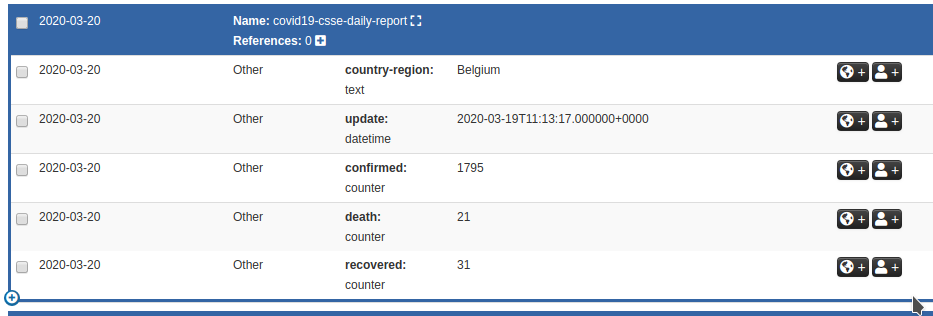
\includegraphics[width=1.00\linewidth]{covidobject.png}
    We are rapidly building new models for the different COVID-19 related information sources
\end{frame}

\begin{frame}
     \frametitle{What kind of information sharing communities exist relying on MISP?}
     \begin{itemize}
       \item {\bf A plethora of "cyber security"-related} communities in CSIRTs, SOC and private exchange groups
       \item Specific {\bf financial} sharing communities in the banking sector
        \item {\bf Border control information} sharing communities
        \item {\bf Vulnerability disclosure} sharing communities
        \item {\bf Intelligence community} sharing community
     \end{itemize}
\end{frame}

\begin{frame}
  \frametitle{Contact us if you want to build your sharing community}
  \begin{itemize}
    \item \url{https://www.misp-project.org/}
    \item \url{https://www.misp-standard.org/}
    \item \url{https://github.com/MISP}
    \item \url{info@misp-project.org}
    \item \url{https://twitter.com/MISPProject}
  \end{itemize}
\end{frame}


